\let\negmedspace\undefined
\let\negthickspace\undefined
\documentclass[journal,12pt,onecolumn]{IEEEtran}
\usepackage{cite}
\usepackage{amsmath,amssymb,amsfonts,amsthm}
\usepackage{algorithmic}
\usepackage{graphicx}
\graphicspath{{./figs/}}
\usepackage{textcomp}
\usepackage{xcolor}
\usepackage{txfonts}
\usepackage{listings}
\usepackage{enumitem}
\usepackage{mathtools}
\usepackage{gensymb}
\usepackage{comment}
\usepackage{caption}
\usepackage[breaklinks=true]{hyperref}
\usepackage{tkz-euclide} 
\usepackage{listings}
\usepackage{gvv}                                        
%\def\inputGnumericTable{}                                 
\usepackage[latin1]{inputenc}     
\usepackage{xparse}
\usepackage{color}                                            
\usepackage{array}
\usepackage{longtable}                                       
\usepackage{calc}                                             
\usepackage{multirow}
\usepackage{multicol}
\usepackage{hhline}                                           
\usepackage{ifthen}                                           
\usepackage{lscape}
\usepackage{tabularx}
\usepackage{array}
\usepackage{float}
\newtheorem{theorem}{Theorem}[section]
\newtheorem{problem}{Problem}
\newtheorem{proposition}{Proposition}[section]
\newtheorem{lemma}{Lemma}[section]
\newtheorem{corollary}[theorem]{Corollary}
\newtheorem{example}{Example}[section]
\newtheorem{definition}[problem]{Definition}
\newcommand{\BEQA}{\begin{eqnarray}}
\newcommand{\EEQA}{\end{eqnarray}}
\newcommand{\define}{\stackrel{\triangle}{=}}
\theoremstyle{remark}
\newtheorem{rem}{Remark}

\begin{document}

\title{12.381}
\author{ee25btech11056 - Suraj.N}
\maketitle
\renewcommand{\thefigure}{\theenumi}
\renewcommand{\thetable}{\theenumi}

\begin{document}

\textbf{Question :} Consider the matrix

\begin{align*}
\vec{A} = \myvec{4 & 0 \\ 0 & 4}
\end{align*}
Which one of the following vectors is \textbf{NOT} a valid eigenvector of the above matrix?

\begin{enumerate}
\begin{multicols}{4}
\item $\myvec{1\\0}$
\item $\myvec{-2\\1}$
\item $\myvec{4\\-3}$
\item $\myvec{0\\0}$
\end{multicols}
\end{enumerate}

\textbf{Solution :}

\begin{table}[h!]
  \centering
  \begin{tabular}{|c|c|}
\hline
\textbf{Name} & \textbf{Value} \\ \hline
$\vec{A}$ & $\myvec{2 & 1 \\0 & 3}$ \\ \hline
\end{tabular}

  \caption*{Table : Matrix}
  \label{12.381}
\end{table}

Since $\vec{A}$ is diagonal, its eigenvalues are the diagonal entries.

\begin{align}
\lambda_1 = 4,\quad \lambda_2 = 4
\end{align}

To find eigenvectors, we solve:

\begin{align}
  (\vec{A}-\lambda\vec{I})\vec{v} = \vec{0}
\end{align}

For $\lambda = 4$:

\begin{align}
  \vec{A}-4\vec{I} &= \myvec{4 & 0 \\ 0 & 4} - \myvec{4 & 0 \\ 0 & 4} \\
&= \myvec{0 & 0 \\ 0 & 0}
\end{align}

So:

\begin{align}
  (\vec{A}-4\vec{I})\vec{v} = \myvec{0 & 0 \\ 0 & 0}\vec{v} = \vec{0}
\end{align}

Thus, every $\vec{v} \in \mathbb{R}^2$ satisfies this equation.  
But an eigenvector must be nonzero.  \\

\textbf{Conclusion:} Any nonzero vector is an eigenvector corresponding to $\lambda=4$.  
The zero vector $\myvec{0\\0}$ is \textbf{not} a valid eigenvector.

\pagebreak

\begin{figure}[h!]
  \centering
  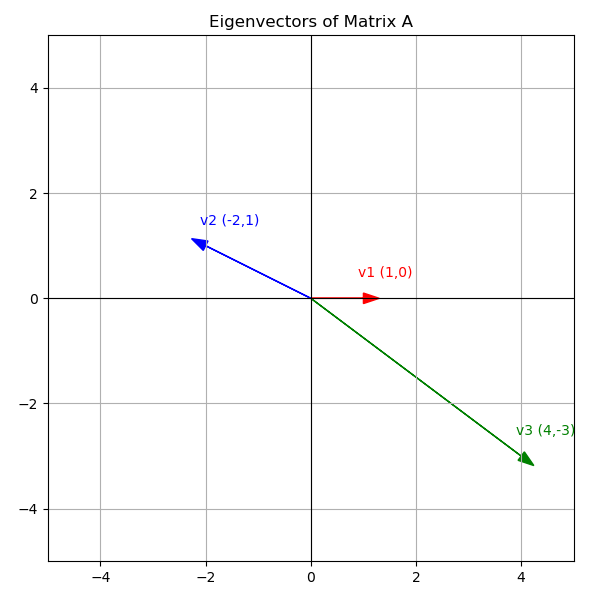
\includegraphics[width=0.7\columnwidth]{figs/eigenvectors.png} 
   \caption*{Fig : Eigen Vectors}
  \label{Fig1}
\end{figure}

\end{document}

